% =====================================================================
%  FICHE DE LECTURE -- Chapitre 3 : Estimation et inférence bayésiennes
%  EPD-SDIA-4112 -- Master 1 SDIA -- ENSPD (Université de Douala)
%  Cas d'étude fil conducteur : TransLog Cameroun SA
%  Durée : 4 h en autonomie complète
%  Tous les chiffres proviennent de src/fiche_ch3_cameroun.py (exécuté)
%  -> figures/key_numbers_fiche_ch3.json
% =====================================================================
\documentclass[11pt,a4paper]{article}
\usepackage[margin=2.2cm]{geometry}
\usepackage[french]{babel}
\usepackage{fontspec}
\setmainfont{Cambria}
\usepackage{amsmath,amssymb}
\usepackage{graphicx}
\usepackage{booktabs}
\usepackage{enumitem}
\usepackage{xcolor}
\usepackage[most]{tcolorbox}
\usepackage{fancyhdr}
\usepackage{hyperref}
\hypersetup{colorlinks=true, linkcolor=blue!60!black, urlcolor=blue!60!black}
\graphicspath{{../figures/}}

\definecolor{bleuenspd}{HTML}{1F4E79}
\definecolor{vertOK}{HTML}{2E7D32}
\definecolor{rougeAlerte}{HTML}{C0504D}
\definecolor{grisClair}{HTML}{F2F2F2}

% ---------------- encadrés ----------------
\newtcolorbox{contexte}[1][]{colback=grisClair, colframe=bleuenspd,
  fonttitle=\bfseries, title={#1}, breakable}
\newtcolorbox{rappel}[1][]{colback=blue!4, colframe=blue!55!black,
  fonttitle=\bfseries, title={Rappel de cours --- #1}, breakable}
\newtcolorbox{application}[1][]{colback=green!4, colframe=vertOK,
  fonttitle=\bfseries, title={Application au dossier TransLog --- #1}, breakable}
\newtcolorbox{qcmbox}[1][]{colback=yellow!5, colframe=orange!80!black,
  fonttitle=\bfseries, title={QCM --- #1}, breakable}
\newtcolorbox{corrigebox}[1][]{colback=green!6, colframe=vertOK,
  fonttitle=\bfseries, title={Corrigé --- #1}, breakable}
\newtcolorbox{piege}[1][]{colback=red!4, colframe=rougeAlerte,
  fonttitle=\bfseries, title={Piège classique --- #1}, breakable}

\pagestyle{fancy}
\fancyhf{}
\fancyhead[L]{\small EPD-SDIA-4112 --- Statistique bayésienne}
\fancyhead[R]{\small Fiche de lecture Ch.~3 --- 4 h}
\fancyfoot[C]{\small page \thepage}
\renewcommand{\headrulewidth}{0.4pt}

\newcommand{\given}{\,\vert\,}

\begin{document}

% =====================================================================
%  PAGE DE GARDE
% =====================================================================
\begin{titlepage}
\centering

\includegraphics[width=4.2cm]{../assets/logo_enspd.png}\\[4mm]
{\Large École Nationale Supérieure Polytechnique de Douala}\\
{\large Université de Douala --- Département Génie Informatique et Télécommunications}\\[10mm]
{\color{bleuenspd}\rule{\textwidth}{1.2pt}}\\[6mm]
{\LARGE\bfseries Fiche de lecture --- Chapitre 3}\\[4mm]
{\huge\bfseries\color{bleuenspd} Estimation et inférence bayésiennes}\\[6mm]
{\color{bleuenspd}\rule{\textwidth}{1.2pt}}\\[8mm]
{\large\bfseries Étude de cas fil conducteur :}\\[2mm]
{\Large « TransLog Cameroun SA --- sécuriser l'axe Douala--Yaoundé »}\\[10mm]

\begin{tabular}{ll}
\toprule
\textbf{Public} & Master 1 SDIA \\
\textbf{Durée totale} & 4 h en autonomie complète \\
\textbf{Prérequis} & Chapitres 1 et 2 (règle de Bayès, lois a priori et a posteriori) \\
\textbf{Matériel} & Cette fiche + les slides du chapitre 3 (sections 3.1 à 3.5) \\
\textbf{Évaluation} & 15 QCM à réponse justifiée (corrigé en fin de fiche) \\
\bottomrule
\end{tabular}

\vspace{8mm}
\begin{contexte}[Comment travailler avec cette fiche]
\begin{itemize}[leftmargin=4mm, itemsep=1mm]
  \item La fiche suit \textbf{un seul dossier d'entreprise} du début à la fin :
        chaque notion du chapitre 3 sert à répondre à une question réelle de la
        direction de TransLog Cameroun SA, transporteur de marchandises sur
        l'axe Douala--Yaoundé.
  \item Chaque section est chronométrée : respecte le minutage, c'est lui qui
        fait la progression.
  \item Les encadrés \textcolor{blue!60!black}{\bfseries rappel} exposent la théorie,
        les encadrés \textcolor{green!50!black}{\bfseries application} la mettent en
        œuvre sur le dossier, les encadrés \textcolor{orange!80!black}{\bfseries QCM}
        vérifient l'assimilation.
  \item \textbf{Ne regarde pas le corrigé avant d'avoir répondu par écrit.}
        Le corrigé justifie chaque bonne réponse et désamorce les pièges.
\end{itemize}
\end{contexte}

\vfill
{\small Enseignante : Dr.\ Noulapeu Ngaffo Armielle --- Statistique bayésienne, M1 SDIA}\\
{\small Document généré à partir de calculs reproductibles (graine 4112).}
\end{titlepage}

\tableofcontents
\newpage

% =====================================================================
%  SECTION 0 -- MISE EN SITUATION (15 min)
% =====================================================================
\section{Mise en situation : le dossier TransLog (15 min)}

\begin{contexte}[Le dossier]
\textbf{TransLog Cameroun SA} est une entreprise de transport routier de
marchandises, basée à Douala. Ses camions font la navette sur l'axe
Douala--Yaoundé, le corridor le plus fréquenté du pays : embouteillages,
revêtements dégradés, trafic dense et hétérogène. Chaque « incident »
(accrochage, sortie de route, retard dommageable) coûte cher : réparation,
immobilisation, pénalités contractuelles, image.

Fin 2024, la direction a déployé un \textbf{programme de formation des
chauffeurs} (éco-conduite, respect des distances, gestion de la fatigue).
Début 2026, le directeur des opérations pose quatre questions, auxquelles
tu vas répondre en tant que \textbf{consultant·e data-science} au fil de
cette fiche :
\begin{enumerate}[leftmargin=5mm, itemsep=1mm]
  \item \textbf{Volet 1 (Q1)} --- après formation, quel est le taux d'incidents
        d'une livraison ? Quel chiffre unique donner au directeur ?
  \item \textbf{Volet 2 (Q2)} --- avec quel niveau de certitude peut-on affirmer
        que le taux est descendu sous le seuil contractuel de 10~\% ?
  \item \textbf{Volet 3 (Q3)} --- que peut-on prédire pour les livraisons
        à venir, et le modèle est-il digne de confiance ?
  \item \textbf{Volet 4 (Q4)} --- le nombre d'incidents mensuels dépend-il du
        volume de trafic ? Peut-on prévoir les mois à fort risque ?
\end{enumerate}
\end{contexte}

\begin{application}[Les données dont tu disposes]
\begin{itemize}[leftmargin=4mm, itemsep=0.5mm]
  \item \textbf{Historique avant formation} : sur 1~000 livraisons, 148 incidents
        (taux $\approx$ 14,8~\%). C'est tout ce qu'on sait du « passé ».
  \item \textbf{Audit post-formation} : 200 livraisons contrôlées, 9 incidents.
  \item \textbf{Comptage mensuel} des incidents sur 6 mois d'exploitation.
  \item \textbf{Facturation} des 15 derniers incidents (coût de chacun).
  \item \textbf{12 mois de données} trafic (milliers de tonnes transportées) vs
        nombre d'incidents du mois.
\end{itemize}
Toutes les valeurs ci-dessous proviennent d'un script reproductible
(\texttt{src/fiche\_ch3\_cameroun.py}, graine 4112) : tu peux rejouer chaque calcul.
\end{application}

% =====================================================================
%  SECTION 1 -- VOLET 1 : ESTIMATEURS PONCTUELS (50 min)
% =====================================================================
\section{Volet 1 --- Quel chiffre unique donner ? Estimateurs ponctuels (50 min)}

\begin{rappel}[Section 3.1 : de la loi a posteriori à l'estimateur]
Le posterior $p(\theta \given y)$ résume \emph{tout} ce qu'on sait sur $\theta$.
Mais un décideur veut \textbf{un chiffre}. Choisir ce chiffre = choisir un
\textbf{estimateur}, et le choix se justifie par une \textbf{fonction de perte}
$L(\hat\theta, \theta)$ qui mesure ce que coûte une erreur :
\begin{itemize}[leftmargin=4mm, itemsep=0.5mm]
  \item \textbf{perte quadratique} $L_2 = (\hat\theta - \theta)^2$
        $\;\Rightarrow\;$ l'estimateur optimal est la \textbf{moyenne} a posteriori
        $\mathbb{E}[\theta \given y]$ ;
  \item \textbf{perte absolue} $L_1 = \lvert \hat\theta - \theta \rvert$
        $\;\Rightarrow\;$ la \textbf{médiane} a posteriori ;
  \item \textbf{perte en « 0--1 »} $L_0$ (erreur si $\hat\theta \ne \theta$)
        $\;\Rightarrow\;$ le \textbf{mode} a posteriori (MAP).
\end{itemize}
Trois perte différentes $\Rightarrow$ trois chiffres différents : il n'y a pas
de « bon » estimateur en soi, seulement un estimateur \emph{adapté à la décision}.
\end{rappel}

\begin{application}[Volet 1 : construire le posterior de TransLog]
\textbf{Étape 1 --- le prior.} L'historique interne (148 incidents pour 1~000
livraisons, soit 14,8~\%) est synthétisé dans un prior beta \textbf{informatif}
mais faible : $\theta \sim \text{Beta}(3, 17)$, équivalent à 20 livraisons fictives,
moyenne $3/20 = 15~\%$. Il encode « le passé était mauvais, mais avec une grande
incertitude ».

\textbf{Étape 2 --- la vraisemblance.} L'audit donne $y = 9$ incidents sur
$n = 200$ livraisons : $y \given \theta \sim \text{Binomial}(200, \theta)$.

\textbf{Étape 3 --- le posterior.} Prior beta + vraisemblance binomiale = famille
conjugée : le posterior est \textbf{Beta}$(3+9,\; 17+200-9)$ $=$
\textbf{Beta}(12, 208). Sa moyenne vaut $12/220 \approx \textbf{5,45~\%}$, son
mode $(12-1)/219 \approx \textbf{5,05~\%}$, sa médiane $\approx \textbf{5,32~\%}$.

\textbf{Lecture du graphique :} le prior (bleu) était énormément étalé autour de
15~\% ; les données (rouge) sont très concentrées autour de 4,5~\% ; le posterior
(vert) est écrasé contre les données : les 200 livraisons auditées pèsent
$200/220 \approx 91~\%$ de l'information totale.
\begin{center}
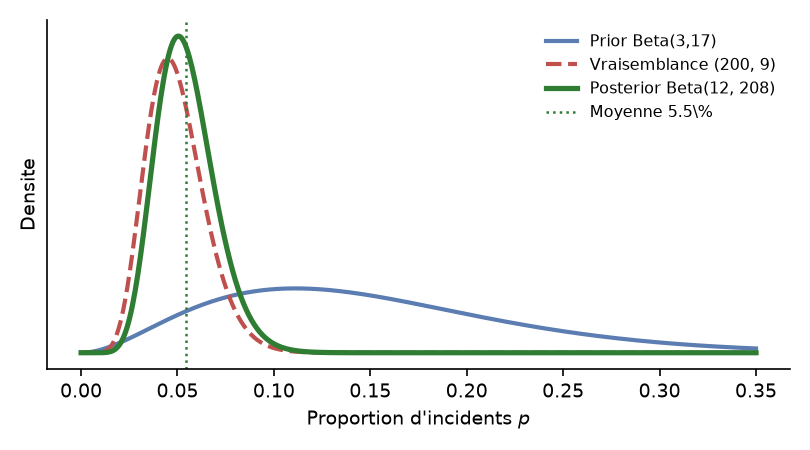
\includegraphics[width=0.72\textwidth]{fiche_ch3_prior_post.png}
\end{center}
\textbf{Réponse au directeur (perte quadratique)} : « le taux d'incidents
post-formation est estimé à \textbf{5,45~\%} » --- contre 14,8~\% avant formation.
\end{application}

\begin{qcmbox}[Questions 1 à 3]
\textbf{Q1.} Sur les seules données de l'audit, l'estimateur du maximum de
vraisemblance (MLE) du taux $p$ vaut :
\begin{enumerate}[label=\Alph*.), leftmargin=8mm, itemsep=0.3mm]
  \item 14,8~\%
  \item 4,5~\%
  \item 5,45~\%
  \item 9~\%
\end{enumerate}

\vspace{2mm}
\textbf{Q2.} Le posterior est Beta(12, 208). Si la direction perd de l'argent
proportionnellement à l'\emph{erreur au carré} (perte quadratique $L_2$),
l'estimateur à donner est :
\begin{enumerate}[label=\Alph*.), leftmargin=8mm, itemsep=0.3mm]
  \item le mode $\approx$ 5,05~\%
  \item la médiane $\approx$ 5,32~\%
  \item la moyenne $\approx$ 5,45~\%
  \item le MLE $\approx$ 4,5~\%
\end{enumerate}

\vspace{2mm}
\textbf{Q3.} Dans le posterior Beta(12, 208) issu du prior Beta(3, 17) et de
200 livraisons auditées, quelle est la part de l'information qui vient
des \emph{données} ?
\begin{enumerate}[label=\Alph*.), leftmargin=8mm, itemsep=0.3mm]
  \item $\approx 9~\%$
  \item $\approx 50~\%$
  \item $\approx 91~\%$
  \item $\approx 99~\%$
\end{enumerate}
\end{qcmbox}

\begin{piege}[Questions 1 à 3]
\begin{itemize}[leftmargin=4mm, itemsep=0.5mm]
  \item \textbf{Q1 vs Q2} : le MLE (4,5~\%) n'est \emph{pas} l'estimateur
        bayésien. Il ignore le prior et ne correspond à aucune fonction de
        perte du cours. Ne jamais confondre « meilleure donnée brute » et
        « décision optimale ».
  \item \textbf{Q2} : la correspondance perte $\to$ estimateur est le cœur de la
        section 3.1 : $L_2 \to$ moyenne, $L_1 \to$ médiane, $L_0 \to$ mode.
        Attention : pour un posterior \emph{asymétrique} (comme ici, queue à
        droite), les trois chiffres diffèrent --- l'écart moyenne--mode vaut
        ici $\approx$ 0,41 point.
  \item \textbf{Q3} : la part des données se lit directement sur les
        « effectifs fictifs » : $200/(200+20) = 91~\%$. Plus le prior est
        faible (peu d'effectifs fictifs), plus les données dominent.
\end{itemize}
\end{piege}

% =====================================================================
%  SECTION 2 -- VOLET 2 : INTERVALLES DE CREDIBILITE (50 min)
% =====================================================================
\section{Volet 2 --- Jusqu'où va notre certitude ? Intervalles de crédibilité (50 min)}

\begin{rappel}[Section 3.2 : les trois intervalles bayésiens]
Un chiffre unique cache l'incertitude. Le remède : un \textbf{intervalle de
crédibilité} au niveau 95~\%, défini \emph{directement sur le posterior} :
\begin{itemize}[leftmargin=4mm, itemsep=0.5mm]
  \item \textbf{intervalle à queue égale} : bornes aux quantiles 2,5~\% et
        97,5~\% du posterior. Simple, symétrique en probabilité.
  \item \textbf{HDI (\emph{Highest Density Interval})} : l'intervalle de
        \textbf{largeur minimale} contenant 95~\% de la masse. Toute valeur
        dedans est plus plausible que toute valeur dehors. Intéressant quand
        le posterior est asymétrique.
  \item \textbf{intervalle unilatéral} : une seule borne, quand la question est
        du type « sommes-nous sûrs que $\theta < \theta_{\text{seuil}}$ ? ».
\end{itemize}
La \textbf{différence fondamentale} avec l'IC fréquentiste : l'intervalle
bayésien porte une phrase du type « $P(\theta \in I \given y) = 0{,}95$ » ---
c'est une probabilité \emph{sur le paramètre}, après avoir vu les données.
L'IC fréquentiste de Wald $\hat\theta \pm 1{,}96\,s/\sqrt{n}$ repose sur
l'approximation normale et ne dit rien de $\theta$ lui-même, seulement
de la procédure sur le long terme.
\end{rappel}

\begin{application}[Volet 2 : le contrat impose 10~\% maximum]
Le contrat signé par TransLog avec ses clients industriels stipule : le taux
d'incidents doit rester \textbf{inférieur à 10~\%}. Le juridique demande :
« êtes-vous sûr à 95~\% que la formation a mis l'entreprise sous ce seuil ? »

\textbf{Intervalle à queue égale :} $P(p \in [2{,}86~\%,\; 8{,}81~\%]) = 95~\%$.
\textbf{HDI 95~\% :} $[2{,}65~\%,\; 8{,}50~\%]$, légèrement plus étroit ---
posterior asymétrique oblige. \textbf{Test unilatéral :}
$P(p < 10~\% \given y) = \textbf{99,4~\%} \gg 95~\%$.

\textbf{Comparaison fréquentiste :} l'IC de Wald $\hat p \pm 1{,}96\sqrt{\hat p(1-\hat p)/n}$
donne $[1{,}63~\%,\; 7{,}37~\%]$ : intervalle plus décalé vers le bas (il est
centré sur le MLE 4,5~\%, pas sur la moyenne posterior 5,45~\%), construit sans
prior, et sans interprétation probabiliste directe sur $p$.

\textbf{Réponse au juridique} : « Oui --- la probabilité a posteriori que le
taux soit sous 10~\% est de 99,4~\%. Le seuil contractuel est respecté. »

\begin{center}
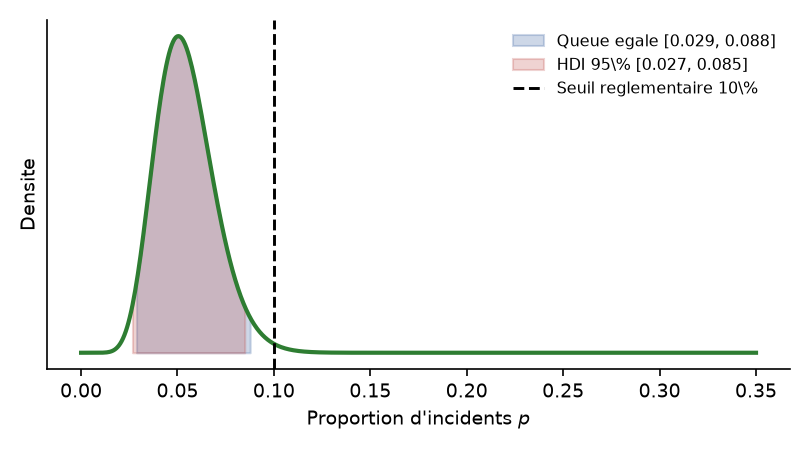
\includegraphics[width=0.72\textwidth]{fiche_ch3_intervalles.png}
\end{center}
\end{application}

\begin{qcmbox}[Questions 4 à 6]
\textbf{Q4.} Pour le posterior Beta(12, 208), quel intervalle à 95~\% est le
\emph{plus court} ?
\begin{enumerate}[label=\Alph*.), leftmargin=8mm, itemsep=0.3mm]
  \item l'intervalle à queue égale
  \item le HDI
  \item ils sont identiques
  \item cela dépend de l'échantillon, pas de la méthode
\end{enumerate}

\vspace{2mm}
\textbf{Q5.} Le contrat exige $P(p < 10~\%) \ge 95~\%$ après observation. La
conclusion de l'inférence bayésienne est :
\begin{enumerate}[label=\Alph*.), leftmargin=8mm, itemsep=0.3mm]
  \item l'exigence est satisfaite ($P \approx 99{,}4~\%$)
  \item l'exigence n'est pas satisfaite
  \item impossible à conclure avec 200 livraisons
  \item cela dépend de l'IC de Wald
\end{enumerate}

\vspace{2mm}
\textbf{Q6.} L'IC fréquentiste de Wald $[1{,}6~\%;\; 7{,}4~\%]$ est plus
\emph{décalé vers le bas} que l'intervalle bayésien $[2{,}9~\%;\; 8{,}8~\%]$.
La raison principale est :
\begin{enumerate}[label=\Alph*.), leftmargin=8mm, itemsep=0.3mm]
  \item Wald est un estimateur biaisé par construction
  \item Wald est centré sur le MLE $\hat p = 4{,}5~\%$, alors que le bayésien
        est centré sur la moyenne posterior (5,45~\%), tirée vers le haut par
        le prior historique
  \item le prior est trop fort
  \item $n = 200$ est trop petit pour Wald
\end{enumerate}
\end{qcmbox}

\begin{piege}[Questions 4 à 6]
\begin{itemize}[leftmargin=4mm, itemsep=0.5mm]
  \item \textbf{Q4} : pour un posterior symétrique (normal), queue égale $=$ HDI.
        Ici la distribution est asymétrique, donc le HDI est plus court ---
        mais de très peu ($\approx$ 0,06 point de largeur). Retenir : le HDI
        est \emph{toujours} $\le$ en largeur à l'intervalle à queue égale.
  \item \textbf{Q5} : c'est toute la puissance de la section 3.2 --- une question
        réglementaire (« sommes-nous sous le seuil ? ») appelle un intervalle
        \textbf{unilatéral} et un calcul de probabilité directe
        $P(p < \text{seuil} \given y)$, pas une danse d'hypothèses.
  \item \textbf{Q6} : le prior de TransLog (15~\% d'historique) \emph{tire vers
        le haut} le posterior. Wald, lui, ne connaît que l'échantillon.
        Aucune des deux approches n'est « plus vraie » : elles répondent à des
        questions différentes.
\end{itemize}
\end{piege}

% =====================================================================
%  SECTION 3 -- VOLET 3 : PREDICTION A POSTERIORI (50 min)
% =====================================================================
\section{Volet 3 --- Que va-t-il se passer ? Prédiction a posteriori (50 min)}

\begin{rappel}[Section 3.3 : prédire une observation future]
L'estimation regarde le passé ; la \textbf{prédiction} regarde l'avenir. La
\textbf{loi prédictive a posteriori} intègre l'incertitude sur $\theta$ :
\[
p(\tilde y \given y) \;=\; \int p(\tilde y \given \theta)\; p(\theta \given y)\; d\theta
\]
En pratique on \textbf{simule} : tirer $\theta^{(s)} \sim p(\theta \given y)$,
puis $\tilde y^{(s)} \sim p(\tilde y \given \theta^{(s)})$. Pour le modèle
beta-binomial de TransLog, la loi prédictive d'une proportion sur $m$
futures livraisons est une \textbf{bêta-binomiale} de paramètres
$(m, a_{\text{post}}, b_{\text{post}})$ --- plus étalée qu'une binomiale
utilisant le seul chiffre $\hat p$, car elle ajoute l'incertitude sur $p$.

\textbf{Posterior predictive check (PPC)} : on simule des jeux de données
\emph{entiers} sous le modèle et on compare à la donnée observée. Si
$y_{\text{obs}}$ tombe dans la masse des simulations, le modèle est cohérent ;
sinon, le modèle (ou le prior) est à rejeter.
\end{rappel}

\begin{application}[Volet 3 : quels risques pour les prochains jours ?]
Le directeur des opérations planifie les tournées de la semaine : « sur les
\textbf{10 prochaines livraisons}, combien d'incidents dois-je budgéter ? »

\textbf{Loi prédictive :} bêta-binomiale de paramètres $(10,\, 12,\, 208)$.
Résultats clés :
\begin{itemize}[leftmargin=4mm, itemsep=0.5mm]
  \item $P(\text{zéro incident sur 10}) = \textbf{57,7~\%}$
  \item $P(\text{au plus 1 incident}) = \textbf{89,7~\%}$
  \item $P(\text{zéro incident sur 20}) = \textbf{34,1~\%}$ --- la série parfaite
        est \emph{rare} même avec un bon taux.
\end{itemize}
\textbf{PPC} : en simulant 10~000 audits de 200 livraisons sous le posterior,
l'intervalle central à 95~\% du nombre d'incidents simulés est $[\,8\,;\,21\,]$.
L'audit observé ($y_{\text{obs}} = 9$) est \textbf{dans} cet intervalle : le
modèle n'est pas rejeté.

\textbf{Réponse au directeur} : « budgétez comme si $\approx 6~\%$ des
livraisons pouvaient avoir un incident ; la semaine zéro incident est
plausible (58~\%) mais loin d'être garantie. »

\begin{center}
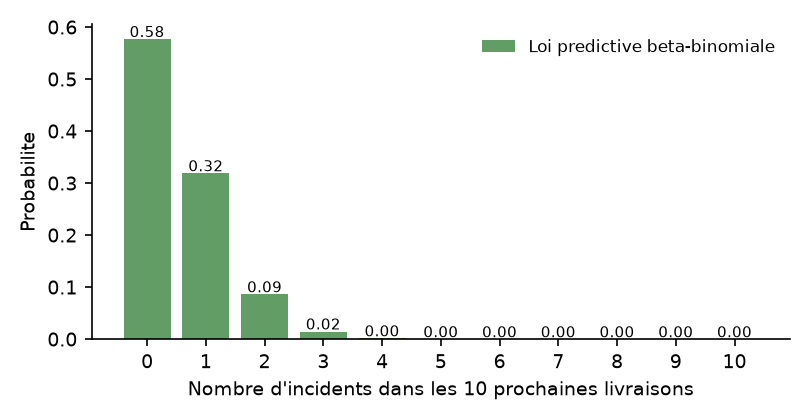
\includegraphics[width=0.66\textwidth]{fiche_ch3_prediction.png}
\end{center}
\end{application}

\begin{qcmbox}[Questions 7 et 8]
\textbf{Q7.} La probabilité qu'aucune des 10 prochaines livraisons n'ait
d'incident vaut :
\begin{enumerate}[label=\Alph*.), leftmargin=8mm, itemsep=0.3mm]
  \item 4,5~\% (le MLE au carré : $0{,}955^{10}$)
  \item 34,1~\%
  \item 57,7~\%
  \item 89,7~\%
\end{enumerate}

\vspace{2mm}
\textbf{Q8.} Le PPC simule 10~000 audits fictifs de 200 livraisons ; 95~\% des
simulations donnent entre 8 et 21 incidents, et l'audit réel compte 9. Que
conclut-on ?
\begin{enumerate}[label=\Alph*.), leftmargin=8mm, itemsep=0.3mm]
  \item le modèle est rejeté : 9 est trop bas
  \item le modèle est cohérent : l'observation est dans la masse prédictive
  \item il faut refaire l'audit
  \item le prior a biaisé la simulation
\end{enumerate}
\end{qcmbox}

\begin{piege}[Questions 7 et 8]
\begin{itemize}[leftmargin=4mm, itemsep=0.5mm]
  \item \textbf{Q7} : le réflexe erroné consiste à brancher le seul chiffre
        $\hat p$ dans une binomiale ($0{,}955^{10} \approx 63~\%$). La vraie
        loi prédictive bêta-binomiale donne 57,7~\% : elle est \textbf{plus
        prudente}, car elle additionne l'incertitude sur $p$ à la variabilité
        binomiale. C'est exactement ce que mesure le chapitre.
  \item \textbf{Q7 bis} : attention, $P(\text{zéro sur 20}) = 34{,}1~\%$, pas
        $57{,}7~\%^2$ : les événements ne sont pas indépendants quand $p$
        lui-même est incertain.
  \item \textbf{Q8} : le PPC ne « valide » pas le modèle au sens formel ; il
        cherche une \textbf{incompatibilité} flagrante. Ici $y_{\text{obs}} = 9$
        est bien dans $[8; 21]$ : pas de signal d'alarme, mais le check doit
        être refait à chaque nouveau lot de données.
\end{itemize}
\end{piege}

% =====================================================================
%  SECTION 4 -- VOLET 4 : CAS APPLIQUES (60 min)
% =====================================================================
\section{Volet 4 --- Trois modèles, trois questions d'entreprise (60 min)}

\subsection{Volet 4a --- Incidents mensuels : modèle Gamma--Poisson (20 min)}

\begin{rappel}[Section 3.4, cas Gamma--Poisson]
Les \textbf{comptages} (incidents par mois, pannes par semaine) suivent une
Poisson$(\lambda)$. En prior gamma (famille conjuguée), si
$\lambda \sim \text{Gamma}(\alpha_0, \beta_0)$ et qu'on observe $n$ mois de
comptages $y_1, \dots, y_n$, alors :
\[
\lambda \given y \sim \text{Gamma}\bigl(\alpha_0 + \textstyle\sum y_i,\;
\beta_0 + n\bigr)
\]
La prédiction d'un nouveau comptage est une \textbf{binomiale négative} de
paramètres $(\alpha_0 + \sum y_i,\; \frac{\beta_0 + n}{\beta_0 + n + 1})$.
\end{rappel}

\begin{application}[Volet 4a : les six mois post-formation]
Comptages mensuels d'incidents : $y = (5,\, 8,\, 16,\, 4,\, 5,\, 6)$ ---
soit 44 incidents en 6 mois, MLE $\hat\lambda = 44/6 = \textbf{7,33}$.
On remarque un mois à 16 incidents (surcharge saisonnière autour des fêtes).

\textbf{Prior} : la logistique estime « environ 5 incidents par mois » avec une
incertitude de $\pm 2$ : $\lambda \sim \text{Gamma}(6,\, 1{,}2)$ (moyenne 5).

\textbf{Posterior} : Gamma$(6+44,\; 1{,}2+6) = $ \textbf{Gamma}(50,\, 7{,}2).
Moyenne $50/7{,}2 = \textbf{6,94}$, médiane $\approx 6{,}90$,
IC 95~\% $= [5{,}15;\; 9{,}00]$, HDI $= [5{,}05;\; 8{,}88]$.

\textbf{Deux questions de gestion :}
\begin{itemize}[leftmargin=4mm, itemsep=0.5mm]
  \item « $\lambda$ dépasse-t-il 10 ? » : $P(\lambda > 10) = \textbf{0{,}26~\%}$
        --- on peut exclure ce scénario catastrophique.
  \item « le mois prochain dépassera-t-il 12 incidents ? » :
        $P(\tilde y > 12) = \textbf{3{,}4~\%}$ --- possible mais peu probable,
        à surveiller.
\end{itemize}

\begin{center}
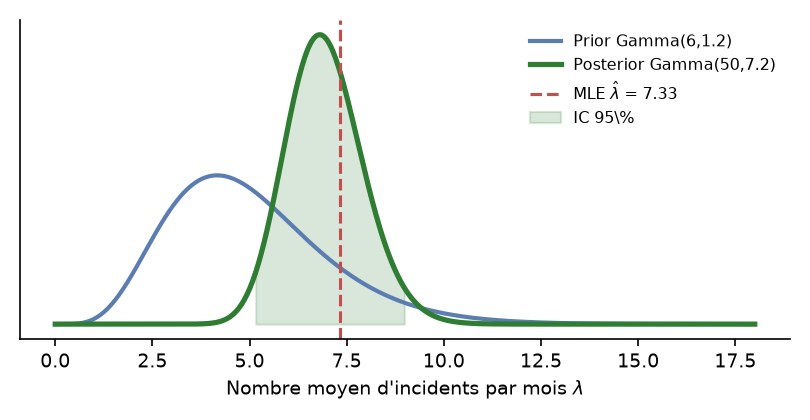
\includegraphics[width=0.68\textwidth]{fiche_ch3_gamma.png}
\end{center}
\end{application}

\begin{qcmbox}[Question 9]
\textbf{Q9.} Avec le prior Gamma(6, 1.2) et 44 incidents en 6 mois, la moyenne
a posteriori de $\lambda$ vaut :
\begin{enumerate}[label=\Alph*.), leftmargin=8mm, itemsep=0.3mm]
  \item $44/6 \approx 7{,}33$
  \item $50/7{,}2 \approx 6{,}94$
  \item $5{,}0$ (le prior)
  \item $\approx 8{,}0$
\end{enumerate}
\end{qcmbox}

\begin{piege}[Question 9]
La moyenne posterior d'une Gamma-Poisson \textbf{n'est pas} le MLE. C'est une
moyenne pondérée entre prior (5,0) et MLE (7,33), pondérée par leurs effectifs
fictifs respectifs ($6$ vs $44$) : $\frac{6 \cdot 5 + 44 \cdot 7{,}33}{50} = 6{,}94$.
Avec $n = 6$ mois seulement, le prior pèse encore $\approx 12~\%$ --- c'est voulu :
le mois à 16 incidents ne doit pas écraser seul l'estimation.
\end{piege}

\subsection{Volet 4b --- Coût d'un incident : modèle Normal--Normal (20 min)}

\begin{rappel}[Section 3.4, cas Normal--Normal]
Pour une \textbf{moyenne} de données continues (coût, durée, prix), si l'écart-type
$\sigma$ est (approximativement) connu et que le prior est normal, tout est
\textbf{conjugue normal} :
\[
\mu \given y \;\sim\; \mathcal{N}\!\left(
\underbrace{w\,\mu_0 + (1-w)\,\bar y}_{\text{moyenne postérieure}},\;
\underbrace{\frac{\sigma^2/n \cdot \tau_0^2}{\sigma^2/n + \tau_0^2}}_{\text{variance postérieure}}
\right), \qquad
w = \frac{\sigma^2/n}{\sigma^2/n + \tau_0^2}
\]
$w$ est le \textbf{poids du prior} : plus les données sont nombreuses ou plus le
prior est incertain ($\tau_0$ grand), plus $w \to 0$ et plus les données dominent.
\end{rappel}

\begin{application}[Volet 4b : combien coûte réellement un incident ?]
La comptabilité facture les 15 derniers incidents (en milliers de FCFA) :
moyenne $\bar y = \textbf{41,9}$, écart-type $s = \textbf{9,2}$,
erreur-type $s/\sqrt{15} = \textbf{2,4}$.

\textbf{Prior} : le service logistique estime « autour de 50 kFCFA », mais
\emph{très} incertain : $\mu \sim \mathcal{N}(50,\, 15^2)$.

\textbf{Posterior} : poids du prior $w = \frac{2{,}4^2}{2{,}4^2 + 15^2} \approx 2{,}5~\%$
$\Rightarrow$ les données pèsent 97,5~\%. Moyenne postérieure :
\[
\mu_{\text{post}} = 0{,}025 \times 50 + 0{,}975 \times 41{,}9 = \textbf{42,1 kFCFA},
\qquad \text{IC 95~\%} = [37{,}5;\; 46{,}7].
\]
\textbf{Lecture} : le prior était à la fois \emph{faux} (50 vs 42) et
\emph{inutile} (15 kFCFA d'incertitude contre 2,4 d'erreur-type d'échantillon) :
les données l'écrasent sans douleur. C'est le comportement idéal d'un prior
faible face à un échantillon décent.
\end{application}

\begin{qcmbox}[Question 10]
\textbf{Q10.} Dans le calcul du coût moyen d'un incident, le poids des données
dans la moyenne postérieure est de 97,5~\%. La raison \emph{principale} est :
\begin{enumerate}[label=\Alph*.), leftmargin=8mm, itemsep=0.3mm]
  \item 15 est un échantillon très grand
  \item le prior est très incertain ($\tau_0 = 15$ kFCFA contre une erreur-type
        d'échantillon de 2,4 kFCFA)
  \item l'écart-type empirique est faible
  \item le prior était trop optimiste
\end{enumerate}
\end{qcmbox}

\begin{piege}[Question 10]
La hiérarchie des facteurs est contre-intuitive : ce n'est pas la \emph{taille}
de l'échantillon en soi, c'est le \textbf{rapport entre l'erreur-type
d'échantillon ($s/\sqrt n$) et l'incertitude du prior ($\tau_0$)}. Avec
$\tau_0 = 15$ et $s/\sqrt{15} = 2{,}4$, le rapport est de 6 : le prior ne pèse
presque rien. Si $\tau_0$ avait été 0,5 (expert très confiant), il aurait pesé
$\approx 96~\%$ \emph{malgré} les données. Le même $n$ peut donner des
conclusions radicalement différentes selon le prior.
\end{piege}

\subsection{Volet 4c --- Prévoir les mois à risque : régression bayésienne (20 min)}

\begin{rappel}[Section 3.4, régression bayésienne]
En régression linéaire bayésienne, on place un prior sur la \textbf{pente} $\beta$
(ici : combien d'incidents supplémentaires par millier de tonnes transportées).
Avec un prior normal $\beta \sim \mathcal{N}(\mu_0, \tau_0^2)$ et une vraisemblance
normale de pente OLS $\hat\beta$ d'erreur-type $\text{se}(\hat\beta)$, le posterior
est de nouveau \textbf{normal}, avec la même mécanique de pondération que le
cas Normal--Normal. La prédiction à un nouveau $x^\ast$ s'écrit :
\[
\tilde y^\ast \;\sim\; \mathcal{N}(\hat\alpha + \beta_{\text{post}} x^\ast,\;
\sigma^2 + \text{sd}(\beta_{\text{post}})^2 (x^\ast - \bar x)^2)
\]
--- la bande s'\emph{élargit} loin de la moyenne des données : l'incertitude de
pente est amplifiée par l'extrapolation.
\end{rappel}

\begin{application}[Volet 4c : le trafic fait-il payer ?]
Douze mois de données : volume transporté (milliers de tonnes) et incidents du
mois. OLS donne une pente $\hat\beta = \textbf{0{,}093}$ incident par millier de
tonnes, erreur-type $\text{se} = \textbf{0{,}0064}$.

\textbf{Prior} : le bureau d'études affirme « la pente est faible, autour de
0,05, avec une incertitude de 0,02 » : $\beta \sim \mathcal{N}(0{,}05,\, 0{,}02^2)$.

\textbf{Posterior} : poids du prior $w \approx 9{,}3~\%$. Pente postérieure :
\[
\beta_{\text{post}} = \textbf{0{,}089}, \qquad
\text{IC 95~\%} = [0{,}077;\; 0{,}101], \qquad
P(\beta > 0) > 99{,}9~\%.
\]
\textbf{Prédiction} : à 200~kt/mois (pic de trafic prévu), le modèle prévoit
$\approx \textbf{14,7}$ incidents/mois --- le mois le plus risqué de l'année.
\textbf{Réponse au directeur} : « chaque 10 kt supplémentaires coûtent
$\approx 0{,}9$ incident/mois ; planifiez renfort maintenance et pause
obligatoire des équipages sur les mois $> 180$ kt. »

\begin{center}
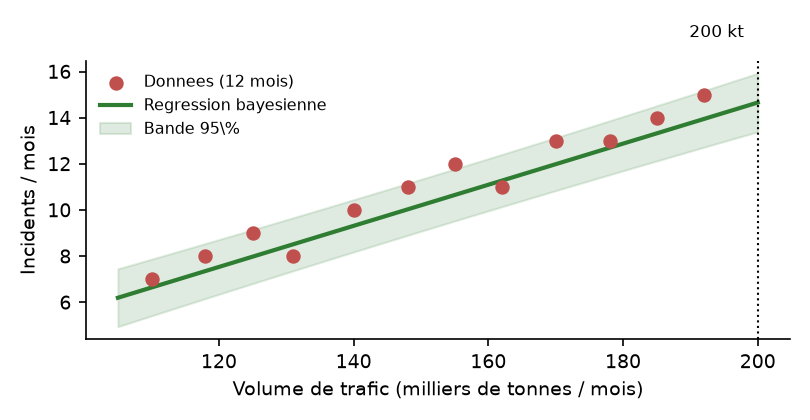
\includegraphics[width=0.68\textwidth]{fiche_ch3_regression.png}
\end{center}
\end{application}

\begin{qcmbox}[Question 11]
\textbf{Q11.} La pente postérieure est 0,089 avec IC 95~\% $= [0{,}077;\, 0{,}101]$.
Que conclut-on sur l'effet du trafic ?
\begin{enumerate}[label=\Alph*.), leftmargin=8mm, itemsep=0.3mm]
  \item l'effet est nul, l'intervalle contient des valeurs proches de 0
  \item l'effet est positif avec une certitude quasi totale ($P > 99{,}9~\%$),
        l'IC est entièrement loin de zéro
  \item il faut 12 mois de données supplémentaires pour conclure
  \item le prior $\mathcal{N}(0{,}05,\, 0{,}02^2)$ domine la conclusion
\end{enumerate}
\end{qcmbox}

\begin{piege}[Question 11]
Deux erreurs à éviter :
\begin{itemize}[leftmargin=4mm, itemsep=0.5mm]
  \item croire qu'un IC « proche de zéro » signifie effet nul : l'IC est
        \textbf{entièrement} au-dessus de zéro, avec une borne basse
        (0,077) déjà très loin de 0 --- c'est la certitude qui compte, pas la
        proximité visuelle.
  \item le prior n'aurait \emph{pas} dominé ici : son poids est de 9,3~\%,
        l'équivalent de 1 mois de données sur 12. Il a \emph{resserré}
        l'estimation (pente postérieure 0,089 vs OLS 0,093) sans la
        renverser.
\end{itemize}
\end{piege}

% =====================================================================
%  SECTION 5 -- VOLET 5 : RISQUE ET SYNTHese (45 min)
% =====================================================================
\section{Volet 5 --- Combien coûte une erreur ? Risque MSE et synthèse (45 min)}

\subsection{Le risque MSE : comparer les estimateurs par simulation (25 min)}

\begin{rappel}[Section 3.4 : risque et MSE]
Un estimateur est bon s'il est \textbf{bon en moyenne sur l'ensemble des
jeux de données possibles} : c'est le \textbf{risque} $\mathbb{E}[(\hat\theta - \theta)^2]$
(l'espérance sur les données, à $\theta$ fixé). En pratique on l'estime par
\textbf{Monte-Carlo} : on simule 500 jeux de données sous un $\theta$ connu, on
calcule $\hat\theta$ bayésien et $\hat\theta$ fréquentiste sur chacun, on compare
les MSE. \textbf{Théorème} : le shrinkage bayésien \emph{domine} le MLE en MSE
quand $n$ est petit \emph{et} que le prior n'est pas trop éloigné de la vérité ;
l'avantage tend vers zéro quand $n \to \infty$.
\end{rappel}

\begin{application}[Volet 5 : la formation vaut-elle son coût ?]
Pour boucler le dossier : le président du conseil se demande si le programme de
formation (2 millions de FCFA/an) doit être généralisé. L'enjeu statistique est
la \textbf{qualité de l'estimation} du taux d'incidents selon la taille de
l'échantillon d'audit. Simulation Monte-Carlo (500 répétitions, $\theta_{\text{vrai}} = 10~\%$,
prior Beta(3, 17) centré à 15~\%) :

\begin{center}
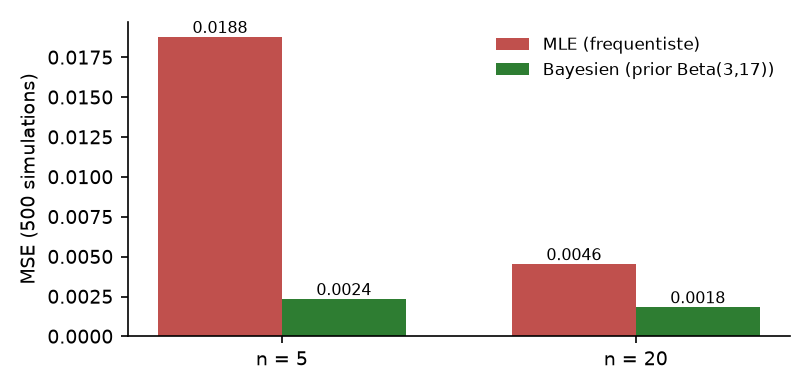
\includegraphics[width=0.62\textwidth]{fiche_ch3_mse.png}
\end{center}

\textbf{À $n = 5$} (audit minimal, 5 livraisons) : le MLE a un MSE de 0,0188 ;
l'estimateur bayésien un MSE de 0,0024 --- \textbf{8 fois meilleur}, car le
shrinkage vers le prior (15~\%) compense l'absence quasi totale de données.
\textbf{À $n = 20$} : le MLE descend à 0,0046, le bayésien à 0,0018 --- encore
un gain, mais plus modeste (ratio 0,41). \textbf{À $n = 400$} (non montré) : les
deux MSE convergent --- le prior ne pèse plus rien.

\textbf{Conclusion business} : le shrinkage bayésien est le meilleur allié quand
on ne peut auditer que quelques livraisons --- exactement la situation des
petites flottes régionales que TransLog veut développer.
\end{application}

\begin{qcmbox}[Questions 12 et 13]
\textbf{Q12.} À $n = 5$, l'estimateur bayésien a un MSE 8 fois plus faible que
le MLE. La raison \emph{principale} :
\begin{enumerate}[label=\Alph*.), leftmargin=8mm, itemsep=0.3mm]
  \item le MLE est biaisé, pas l'estimateur bayésien
  \item le prior, centré à 15~\% quand la vérité est à 10~\%, réduit la variance
        par shrinkage et n'ajoute presque pas de biais
  \item c'est une coïncidence de cette simulation
  \item le MLE sous-estime systématiquement $\theta$
\end{enumerate}

\vspace{2mm}
\textbf{Q13.} Quand $n$ grandit ($n = 20$, puis 400), le ratio
MSE$_{\text{bayésien}}$/MSE$_{\text{MLE}}$ :
\begin{enumerate}[label=\Alph*.), leftmargin=8mm, itemsep=0.3mm]
  \item augmente : le prior finit par nuire
  \item tend vers 1 : les données écrasent le prior, l'avantage s'efface
  \item tend vers 0 : le bayésien devient parfait
  \item reste constant quel que soit $n$
\end{enumerate}
\end{qcmbox}

\begin{piege}[Questions 12 et 13]
\begin{itemize}[leftmargin=4mm, itemsep=0.5mm]
  \item \textbf{Q12} : le gain bayésien à petit $n$ vient de la
        \textbf{décomposition biais-variance} : le MLE a une variance énorme
        ($\theta(1-\theta)/n$ avec $n=5$), le shrinkage bayésien l'écrase en
        échange d'un léger biais (prior à 15~\% vs vérité 10~\%). Le biais
        acheté est minuscule, la variance économisée est massive.
  \item \textbf{Q13} : c'est la réponse théorique clé de la section 3.4 :
        \textbf{l'avantage bayésien est un phénomène de petit échantillon}.
        Avec beaucoup de données, prior et MLE convergent --- ce qui est
        rassurant : la méthode ne devient jamais \emph{pire} que le MLE si le
        prior est raisonnable.
\end{itemize}
\end{piege}

\subsection{Synthèse : les 5 réflexes à emporter (20 min)}

\begin{contexte}[Récapitulatif du dossier TransLog]
\begin{center}
\small
\begin{tabular}{@{}p{3.9cm} p{4.1cm} p{5.4cm}@{}}
\toprule
\textbf{Question business} & \textbf{Outil du chapitre 3} & \textbf{Réponse chiffrée} \\
\midrule
Taux d'incidents post-formation ? & posterior Beta(12, 208), moyenne ($L_2$) & 5,45~\% (MLE : 4,5~\%) \\
Sous le seuil contractuel de 10~\% ? & probabilité unilatérale a posteriori & $P(p<10\%) = 99{,}4~\%$ : oui \\
Zéro incident la semaine prochaine ? & loi prédictive bêta-binomiale & $P = 57{,}7~\%$ sur 10 livraisons \\
Le modèle est-il digne de confiance ? & posterior predictive check & $y_{\text{obs}}=9$ dans $[8; 21]$ : cohérent \\
Incidents par mois ? & posterior Gamma(50, 7.2) & moyenne 6,94, IC 95~\% $[5{,}15;\, 9{,}00]$ \\
Coût moyen d'un incident ? & posterior Normal--Normal & 42,1 kFCFA, IC 95~\% $[37{,}5;\, 46{,}7]$ \\
Effet du trafic sur les incidents ? & régression bayésienne & pente 0,089, $P>0 > 99{,}9~\%$ \\
Généraliser la formation ? & comparaison MSE par Monte-Carlo & bayésien 8$\times$ meilleur à $n=5$ \\
\bottomrule
\end{tabular}
\end{center}

\textbf{Les 5 réflexes} à ancrer avant le chapitre 4 :
\begin{enumerate}[leftmargin=5mm, itemsep=1mm]
  \item \textbf{Un chiffre n'existe pas sans fonction de perte} : moyenne,
        médiane ou mode selon ce que coûte l'erreur (3.1).
  \item \textbf{L'intervalle se choisit selon la question} : queue égale par
        défaut, HDI pour la plausibilité, unilatéral pour un seuil (3.2).
  \item \textbf{La prédiction ajoute toujours de l'incertitude} : jamais de
        binomiale branchée sur $\hat p$ (3.3).
  \item \textbf{Tout modèle se met à l'épreuve} : PPC avant de livrer un
        chiffre au décideur (3.3).
  \item \textbf{Le prior est un allié à petit $n$ et s'efface à grand $n$} :
        c'est un choix de modélisation, pas une faiblesse (3.4).
\end{enumerate}
\end{contexte}

% =====================================================================
%  SECTION 6 -- QCM DE SYNTHESE (25 min)
% =====================================================================
\section{QCM de synthèse --- les réflexes transversaux (25 min)}

\begin{qcmbox}[Questions 14 et 15]
\textbf{Q14.} Pour quelle(s) raison(s) préfère-t-on le HDI à l'intervalle à
queue égale ? (une seule bonne réponse)
\begin{enumerate}[label=\Alph*.), leftmargin=8mm, itemsep=0.3mm]
  \item le HDI est plus court quand le posterior est asymétrique, et toute
        valeur dedans est plus plausible que toute valeur dehors
  \item le HDI garantit une couverture de 95~\% en répétant l'expérience
  \item le HDI est symétrique autour de la moyenne
  \item le HDI est le seul intervalle valide quand $n < 30$
\end{enumerate}

\vspace{2mm}
\textbf{Q15.} TransLog doit trancher : \emph{poursuivre la formation}
(coût 2 MFCFA/an) ou \emph{revenir aux pratiques antérieures}. L'apport
spécifique de l'inférence bayésienne à cette décision est :
\begin{enumerate}[label=\Alph*.), leftmargin=8mm, itemsep=0.3mm]
  \item une réponse définitive : la formation est bonne, point
  \item une loi a posteriori sur $p$ + des probabilités prédictives, qui
        permettent de comparer les espérances de perte des deux décisions
  \item uniquement le MLE du taux d'incidents
  \item rien : la décision appartient au directeur seul
\end{enumerate}
\end{qcmbox}

\begin{piege}[Questions 14 et 15]
\begin{itemize}[leftmargin=4mm, itemsep=0.5mm]
  \item \textbf{Q14} : la couverture en répétition est un concept
        \emph{fréquentiste} --- un HDI bayésien ne promet rien sur la
        répétition, il décrit l'incertitude \emph{après} avoir vu les données.
        Et il n'est symétrique que si le posterior l'est.
  \item \textbf{Q15} : c'est la charnière avec le chapitre 4 (comparaison et
        décision) : l'inférence ne tranche pas à la place du décideur, elle
        \textbf{chiffre les conséquences probabilistes} de chaque option pour
        qu'il puisse calculer des espérances de perte. Relis la question
        centrale du chapitre : « ce chiffre dépend de ce que coûte une erreur ».
\end{itemize}
\end{piege}

% =====================================================================
%  SECTION 7 -- CORRIGE
% =====================================================================
\newpage
\section{Corrigé complet des 15 QCM}

\begin{corrigebox}[Volet 1 --- estimateurs ponctuels]
\textbf{Q1 : B.} Le MLE maximise la vraisemblance binomiale : c'est simplement
$\hat p = y/n = 9/200 = \textbf{4{,}5~\%}$. Aucun prior, aucune fonction de
perte --- c'est la donnée brute, pas la décision.

\textbf{Q2 : C.} La perte quadratique $L_2 = (\hat\theta - \theta)^2$ est
minimisée, en espérance sur le posterior, par la \textbf{moyenne a posteriori} :
$\mathbb{E}[\theta \given y] = a_{\text{post}}/(a_{\text{post}} + b_{\text{post}})
= 12/220 = \textbf{5{,}45~\%}$. Le mode (5,05~\%) répond à la perte en 0--1, la
médiane (5,32~\%) à la perte absolue. Ici, posterior asymétrique, les trois
sont ordonnés : mode $<$ médiane $<$ moyenne.

\textbf{Q3 : C.} Les effectifs fictifs du posterior sont la somme de ceux du
prior et de ceux des données : prior $= 3+17 = 20$ livraisons équivalentes,
données $= 200$. Part des données : $200/220 = \textbf{90{,}9~\%}$. C'est la
raison pour laquelle le posterior est si proche du MLE : le prior de TransLog
est \emph{faible} par rapport à l'audit.
\end{corrigebox}

\begin{corrigebox}[Volet 2 --- intervalles de crédibilité]
\textbf{Q4 : B.} Le HDI est, par construction, l'intervalle de 95~\% de
\textbf{plus courte largeur} : on maximise la densité dedans, donc on inclut
d'abord les valeurs les plus plausibles. Sur le posterior Beta(12, 208)
(asymétrique, queue droite), le HDI $[2{,}65\%;\, 8{,}50\%]$ est plus étroit que
l'intervalle à queue égale $[2{,}86\%;\, 8{,}81\%]$. Les deux contiennent 95~\%
de la masse --- la différence est dans la \emph{forme}, pas dans la couverture.

\textbf{Q5 : A.} La question juridique est unilatérale : « sommes-nous sous
10~\% ? ». On calcule directement $P(p < 0{,}10 \given y) =
\text{cdf}_{\text{Beta}(12,208)}(0{,}10) = \textbf{99{,}4~\%}$, largement
au-dessus du seuil de 95~\%. L'exigence contractuelle est satisfaite avec
une marge confortable --- c'est une réponse probabiliste directe,
impossible à formuler en termes fréquentistes purs.

\textbf{Q6 : B.} Wald est construit autour du MLE $\hat p = 4{,}5~\%$, en
utilisant l'approximation normale de la binomiale \emph{plugg-in} : borne
basse $4{,}5 - 1{,}96\sqrt{\frac{4{,}5 \times 95{,}5}{200}} = 1{,}63~\%$.
L'intervalle bayésien est construit sur le \textbf{posterior} (moyenne
5,45~\%), tiré vers le haut par le prior historique (15~\%). La différence
de centrage ($\approx 1$ point) est le poids résiduel du prior
($200/220 = 91~\%$ des effectifs, il ne reste que 9~\% d'influence).
Ce n'est ni un biais « par construction », ni un problème de taille
d'échantillon.
\end{corrigebox}

\begin{corrigebox}[Volet 3 --- prédiction a posteriori]
\textbf{Q7 : C.} La loi prédictive des $m$ prochaines livraisons après
intégration sur $p$ est la \textbf{bêta-binomiale}$(m, a_{\text{post}},
b_{\text{post}}) = (10, 12, 208)$ :
\[
P(\tilde y = 0) = \frac{B(12,\, 218)}{B(12,\, 208)} \cdot \binom{10}{0}
= \textbf{57{,}7~\%}.
\]
Le réflexe erroné (binomiale branchée sur $\hat p = 0{,}955$) donne
$0{,}955^{10} = 63{,}2~\%$ : \emph{trop optimiste}, car il ignore que $p$
lui-même est incertain. La bêta-binomiale est toujours au moins aussi étalée
que la binomiale plug-in : c'est la correction d'incertitude du chapitre.

\textbf{Q8 : B.} Un PPC \emph{ne rejette pas} le modèle tant que
$y_{\text{obs}}$ tombe dans la masse des simulations. Ici, 95~\% des audits
simulés donnent entre 8 et 21 incidents, et $y_{\text{obs}} = 9$ : parfaitement
cohérent. Remarque : l'intervalle simulé $[8, 21]$ est \emph{plus large} que
l'IC bayésien sur $p$ converti en comptage ($200 \times [2{,}86\%; 8{,}81\%]
= [5{,}7; 17{,}6]$) --- c'est normal, le PPC intègre en plus la variabilité
binomiale \emph{des données autour de $p$}. Retenir : IC sur le paramètre $=$
incertitude de $p$ ; PPC $=$ incertitude de $p$ $+$ bruit d'échantillonnage.
\end{corrigebox}

\begin{corrigebox}[Volet 4 --- les trois modèles appliqués]
\textbf{Q9 : B.} Mise à jour Gamma--Poisson :
$\alpha_{\text{post}} = 6 + 44 = 50$,
$\beta_{\text{post}} = 1{,}2 + 6 = 7{,}2$ ;
moyenne $= \alpha/\beta = 50/7{,}2 = \textbf{6{,}94}$. Le MLE (7,33) et le
prior (5,0) ont été combinés selon leurs effectifs fictifs ($44$ vs $6$) :
\[
\frac{6 \times 5{,}0 + 44 \times 7{,}33}{50} = 6{,}94 \;\checkmark
\]
Le mois à 16 incidents est inclus dans $\sum y_i$ mais son poids est dilué par
les 5 autres mois --- c'est le rôle du prior.

\textbf{Q10 : B.} Le poids du prior dans le posterior Normal--Normal est
$w = \frac{\sigma^2/n}{\sigma^2/n + \tau_0^2}$. Ici
$\sigma^2/n \approx 2{,}4^2 = 5{,}8$ et $\tau_0^2 = 225$ : le rapport est de
$5{,}8/230{,}8 \approx 2{,}5~\%$ de poids au prior, soit 97,5~\% pour les
données. Ce n'est pas la taille de l'échantillon (15 est modeste) mais le
\textbf{ratio} entre l'erreur-type d'échantillon (2,4 kFCFA) et l'incertitude
du prior (15 kFCFA). Avec un expert très confiant ($\tau_0 = 0{,}5$), le prior
aurait pesé 96~\% malgré 15 observations.

\textbf{Q11 : B.} L'IC bayésien à 95~\% de $\beta$ est
$[0{,}077;\, 0{,}101]$, entièrement au-dessus de zéro, avec
$P(\beta > 0) > 99{,}9~\%$ : l'effet du trafic est positif et quasi certain.
Le prior n'a \emph{pas} dominé : poids résiduel de 9,3~\% (ratio entre
$\text{se}(\hat\beta) = 0{,}0064$ et $\tau_0 = 0{,}02$), il a resserré
l'estimation (0,089 vs OLS 0,093) sans la renverser. En outre, la prédiction
à 200 kt (14,7 incidents/mois) montre que l'extrapolation, gérée par le
modèle, augmente l'incertitude --- c'est l'usage correct d'une régression
bayésienne pour la prévision de risque.
\end{corrigebox}

\begin{corrigebox}[Volets 5 et synthèse --- risque et décision]
\textbf{Q12 : B.} Le gain vient de la \textbf{décomposition biais-variance}.
MLE : sans biais, mais variance $\theta(1-\theta)/n$ énorme à $n = 5$
($\approx 0{,}018$), car 5 observations ne peuvent pas estimer précisément
une proportion. Bayésien avec prior Beta(3, 17) (moyenne 0,15) : shrunk vers
0,15, donc biais positif d'environ 0,05 en moyenne --- mais variance
dramatiquement réduite. Le trade-off est largement favorable (MSE 0,0024
contre 0,0188). Notons que le prior, bien que \emph{imparfait} (15~\% vs
vérité 10~\%), reste « dans le bon quartier » : c'est la condition du gain.

\textbf{Q13 : B.} À $n = 20$, le ratio est déjà 0,41 ; à $n = 400$, il
converge vers 1 : les données écrasent le prior, les deux estimateurs
coïncident. \textbf{C'est la conclusion théorique clé} : l'avantage bayésien
est un phénomène de \emph{petit échantillon}, pas une supériorité universelle.
En régime de données abondantes, le prior ne fait plus la différence ---
et c'est très bien ainsi : la méthode ne se retourne jamais contre l'analyste
tant que le prior est raisonnable.

\textbf{Q14 : A.} Deux propriétés du HDI : (i) c'est l'intervalle de 95~\% le
plus court, (ii) toute valeur dedans a une densité supérieure à toute valeur
dehors --- une lecture de « plausibilité » directe. Les propositions B
(couverture en répétition : concept fréquentiste, le HDI n'y engage rien),
C (symétrie : faux en général) et D (validité conditionnelle à $n$ : faux) sont
des pièges classiques de confusion bayésien/fréquentiste.

\textbf{Q15 : B.} L'inférence bayésienne ne tranche pas à la place du décideur.
Elle fournit (i) la loi a posteriori de $p$ ($\Rightarrow$ incertitude
quantifiée sur le taux), (ii) la loi prédictive (impacts futurs), (iii) les
deux ensemble permettent de calculer l'\textbf{espérance de perte} de chaque
décision (« poursuivre » vs « revenir en arrière ») et de choisir celle qui
minimise le risque. C'est le pont vers le chapitre 4 (comparaison et décision)
et l'exact formulation de la question centrale du cours : « ce chiffre dépend
de ce que coûte une erreur ». La réponse D serait exacte pour le \emph{choix
final}, mais pas pour l'\emph{apport} de l'inférence.
\end{corrigebox}

% =====================================================================
%  SECTION 8 -- POUR ALLER PLUS LOIN
% =====================================================================
\section{Pour aller plus loin}

\begin{contexte}[Après la fiche --- avant le chapitre 4]
\begin{itemize}[leftmargin=4mm, itemsep=1mm]
  \item \textbf{Relis les slides} : chapitre 3, sections 3.1 (slides 3--16),
        3.2 (slides 17--26), 3.3 (slides 27--34), 3.4 (slides 35--45),
        3.5 (slides 46--50). Chaque section correspond à un volet de cette fiche.
  \item \textbf{Rejoue les calculs} : le script \texttt{src/fiche\_ch3\_cameroun.py}
        régénère toutes les données du dossier (graine 4112) et les figures.
        Modifie le prior (par exemple $\text{Beta}(10, 10)$) et observe ce qui
        change dans les trois estimateurs --- c'est le meilleur entraînement
        possible sur la sensibilité au prior.
  \item \textbf{Prépare le chapitre 4} : lis la section 4.1 avant le prochain
        cours --- elle pose le cadre décisionnel (fonction de perte, espérance
        de perte, valeur prédictive) dont la Q15 a donné un aperçu.
  \item \textbf{TP de rattrapage} : le notebook \texttt{TP3\_estimation\_inference.ipynb}
        (répertoire \texttt{notebooks/}) te fait refaire toutes ces étapes en
        code, avec les mêmes données.
\end{itemize}
\end{contexte}

\vspace{4mm}
\begin{center}
{\small\itshape Fiche de lecture EPD-SDIA-4112 --- Chapitre 3.\\
Toutes les valeurs citées proviennent de \texttt{figures/key\_numbers\_fiche\_ch3.json},
généré par \texttt{src/fiche\_ch3\_cameroun.py} (graine 4112).}
\end{center}

\end{document}
